\documentclass{article}

\usepackage{fontspec}
\usepackage{fullpage}
\usepackage{graphicx}
\usepackage{multicol}
\usepackage{multirow}
\usepackage{tikz}

\begin{document}

\newfontfamily\swfill{SuttonSignWritingFill.ttf}
\newfontfamily\swline{SuttonSignWritingLine.ttf}
\newcommand{\bul}{\hfil$\bullet$&}
\renewenvironment{glossary}{\begin{multicols}{5}\begin{center}}{\end{center}\end{multicols}}
\setcounter{secnumdepth}{0}
\setlength{\columnseprule}{1pt}

\section{Lesson 1}

\begin{center}
\it
Objectives inspired by, lesson material copied from, vocabulary transcribed from, and sentences and story by Bill Vicars.
No endorsement implied nor given.
\end{center}

\subsection{Objectives}

\begin{tabular}{p{1cm}p{14cm}}
\bul I am able to define the term ASL.\\
\bul I know and can read the common handshapes used in ASL.\\
\bul I am able to read, write, and fingerspell my name in ASL.\\
\bul I am able to read, write, and count to five in ASL.\\
\bul I am able to briefly describe the history of ASL.\\
\bul I am able to briefly describe the history of SignWriting.\\
\bul I am able to briefly state the gist of Deaf Culture.\\
\bul I have a \emph{basic} idea of the meaning of the difference between ASL and Signed English.\\
\bul I have a \emph{basic} idea of the meaning of Pidgin (concat signing).\\
\bul I know which direction to read and write SignWriting.\\
\bul I am able to explain how the glyphs of SignWriting are organized.\\
\bul I have a \emph{basic} idea of how dictionary order works.\\
\bul I know how SignWriting works with left handed signing.\\
\bul I am able to read, recognize, and sign the vocabulary for this lesson.\\
\bul I am able to read, recognize, and sign the practice sentences for this lesson.\\
\bul I am able to read the practice story for this lesson.\\
\bul I have done a practice quiz.\\
\bul I have checked with my instructor regarding how and where to take any graded quizzez.\\
\end{tabular}

\subsection{ASL: A Brief Description}

Let me start by sharing with you \emph{my} definition of ASL:
``American Sign Language is a visually perceived language based on a naturally evolved system of articulated hand gestures and their placement relative to the body, along with non-manual markers such as facial expressions, head movements, shoulder raises, mouth morphemes, and movements of the body.''

Now let's look at a couple of other definitions.
According to \texttt{www.dictionary.com} we have:

\begin{quote}
\textbf{American Sign Language} \textit{n. Abbr.} \textbf{ASL}:
The primary sign language used by deaf and hearing-impaired people in the United States and Canada, devised in part by Thomas Hopkins Gallaudet on the basis of sign language in France.
Also called \textbf{Ameslan}.
\end{quote}

A quick trip to Merriam-Webster's Collegiate Dictionary (\texttt{www.m-w.com}) and we get:

\begin{tabular}{rp{10cm}}
Main Entry:&\textbf{American Sign Language}\\
Function:&\emph{noun}\\
Date:&1960\\
\textbf{:}&a sign language for the deaf in which meaning is conveyed by a system of articulated hand gestures and their placement relative to the upper body\\
\end{tabular}

I've also seen this definition show up in \emph{many} places:

\begin{quote}
``American Sign Language is a visual-gestural language used by 500,000 members of the North American Deaf community.''
\end{quote}

Here is a variation on that same theme:

\begin{quote}
``American Sign Language is a visual-gestural language used primarily by members of the North American Deaf community.''
\end{quote}

Now let's discuss those definitions a bit.

Did you notice the date of that entry from Merriam-Webster?
1960!
ASL hasn't been ``recognized'' as a language for very long has it?
Oh sure, ASL has been used in; America since the early 1800's (and earlier if you include the signing that was being done in America prior to Thomas Gallaudet bringing Laurent Clerc from France), but it wasn't until 1960 that ``experts'' \emph{started} recognizing it as a full-blown autonomous language.

We should say ``at \emph{least}'' 500,000 people use ASL.
That is an \textbf{old} statistic from the 1980's.
My estimate is more along the lines of:
2 million people are using ASL on a daily basis and at least 500,000 of those people are using it as their primary means of communication.
Millions more people know ``some'' sign language and use it ``once in a while.''
For example, a grandmother of a deaf child.
She may have taken a six-week community education course and now she knows just enough to offer her grandson candy and cookies.

``ASL is a visually perceived, gesture-based language.''
That means it is a language that is expressed through the hands and face and is perceived through the eyes.
It isn't just  waving your hands in the air.
If you furrow your eyebrows, tilt your head, glance in a certain direction, twist your body a certain way, puff your cheek, or any number of other ``inflections'' --- you are adding or changing meaning in ASL.
A ``visual gestural'' language carries just as much information as an oral/aural (mouth/ear) language.

Is ASL limited to just the United States and Canada?

No.
ASL is also used \textbf{\emph{in varying degrees}} in the Philippines, Ghana, Nigeria, Chad, Burkina Faso, Gabon, Zaire, Central African Republic, Cote d'Ivoire, Mauritania, Kenya, Madagascar, Benin, Togo, Zimbabwe, Singapore, Hong Kong and many other places.
{\small (Source: Grimes, Barbara F. (editor), (1996). ``Languages of USA'' \emph{Ethnologue: Languages of the World, 13th Edition.} Institute of Linguistics.)}

Is ASL a \textbf{\emph{universal}} language?
Nope.
Not even close.
Those countries I just mentioned also have \emph{their own} signed languages.
For a idea into how non-universal it is, take a look at the number of languages listed on \texttt{https://www.signbank.org/signmaker.html}!
ASL is the dominant signed language in \emph{North America}, plus it is used \emph{to some extent} in quite a few other countries, but it is certainly not understood by Deaf people everywhere.

\subsection{American Sign Language: Handshapes}

A student wrote:
``I was looking at some of the signs, but couldn't tell which way my hands should be facing.
For example one of the versions of the sign pizza uses a `p' handshape.
Is the `P' facing me or the person I'm signing to?''

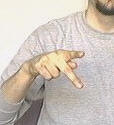
\includegraphics[scale=0.5]{images/handsh1.jpg}
Dr Vicars:
When fingerspelling, in general the palm of your hand faces toward the watcher.
For the sake of comfort your palm is actually pointed a bit off to the right of the person to whom you are spelling.
(Unless you are left handed, then it will be opposite.)

Letters like G, H, and P point a bit off to the right of the person to whom you are signing.
Some signers point these letters almost directly to the left.
Both methods are ``okay.''
Use a position that feels comfortable to you yet is clear to the observer.
In most pictorial sign language dictionaries, unless it says or shows otherwise, you can assume the sign is angled toward the watcher.
It is important to note though that sometimes when you aim a sign at yourself or move a sign toward yourself you are doing so to create additional meaning.
(Mine vs. yours / done to me vs. done to you.)

\subsubsection{A:}

When reading ``letter A'' it will look like B510x508S1f720490x493.
When watching someone else sign you the letter ``A'', it will look like 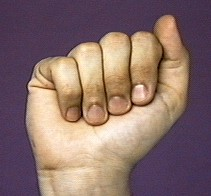
\includegraphics[scale=0.5]{images/a.jpg} to you.
When writing ``letter A'' you should make it look like \tikz{\draw[thick](0,0)rectangle(10pt,10pt);\draw[thick](0,0)--(10pt,10pt);\draw[thick](0,10pt)--(10pt,0);\draw[thick](0,0)--(-5pt,5pt);}.

Don't worry too much about how to read and write ``A'' for now (unless it's in your name).
Just know for now that a filled in area is drawn by using an ``X'' to fill it in and that we will be showing the SignWriting for each of these handshapes along with the picture.

\subsubsection{B:}

``B'' Version 1:
The thumb of the letter ``B'' generally has a ``slight'' bend, but not as much as depicted in most books.
The picture of ``B'' in my \texttt{http://asl.ms} website was taken in a series as I was spelling the ABC's.

You might notice that a ``B'' being produced after an ``A'' tends to have little or no bend.
If you videotape a skilled signer fingerspelling the word ``about'' at \emph{high} speed, the ``B'' will generally have little or no bend in the thumb.
If you video record that same person spelling of the term ``MBA'' the ``B'' will have a very noticeable bend.
The letter B is spelled B507x511S14720493x489 regardless of any signing differences, just like the different sounds for ``L'' are ignored when reading and writing English.
Here's how I do the letter ``B'' in general:

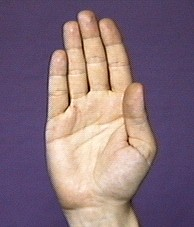
\includegraphics[scale=0.5]{images/b1.jpg}
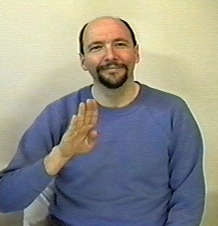
\includegraphics[scale=0.5]{images/b.jpg}

``B'' Version 2:
Some people cross the thumb over the palm.
I don't do it this way because it takes too much effort.
(Hey, I'm not lazy, just efficient.)
This is how most ``books'' show it:
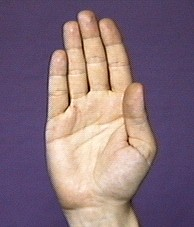
\includegraphics[scale=0.5]{images/b1.jpg}

\begin{quote}
\textbf{Shannon:}
What is a ``b'' palm?
It doesn't relate to signing the letter ``b'' right?

\textbf{DrVicars}:
When used to describe a sign, a ``b'' palm is like the letter ``b'' but you don't have to bend the thumb around onto the palm.
The thumb is just alongside the palm in a natural position, with the fingers touching each other (side by side, extended).
Think of a traffic cop telling oncoming traffic to stop.

\textbf{Shannon}:
Okay that's what I guessed; just wanted to make sure.
\end{quote}

\subsubsection{``Classifier B,'' ``Flat hand,'' or ``B palm.''}

This handshape uses a ``B'' hand with the thumb alongside instead of folded across the palm.
This handshape is used to describe flat, rectangular objects or surfaces.
Examples:
the roof of a house, a sheet of paper, a table, a box $\ldots$

B506x514S15a20494x487 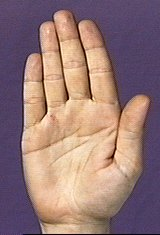
\includegraphics[scale=0.5]{images/flat.jpg}

\subsubsection{C:}

B509x510S16d20492x490 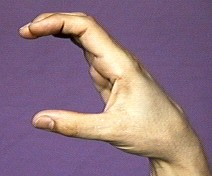
\includegraphics[scale=0.5]{images/c.jpg}

When used as a \textbf{size} and \textbf{shape} specifier this handshape shows things that are round or cylindrical.
Examples: pole, cup, or telescope.
This handshape can also be used to specify placement.
You could show where certain things are in a room.
For example, a TV or a microwave.
To describe a TV or microwave you could use \textbf{index} fingers to trace its outline, or \textbf{b-hands} to show its size and shape.

\subsubsection{D:}

B508x515S10110492x485 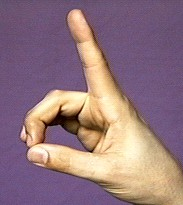
\includegraphics[scale=0.5]{images/d.jpg}

\subsubsection{E:}

B508x508S14a20493x493 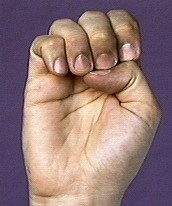
\includegraphics[scale=0.5]{images/e.jpg}

You might see an ``e'' that rests only three fingers on top of the thumb when someone is spelling a name or a word that places the letter ``m'' before the ``e.''
For example: ``James.''

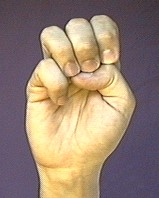
\includegraphics[scale=0.5]{images/e3.jpg}

Or suppose you spell the name ``J-A-N-E?''
The ``E'' might end up looking like this:

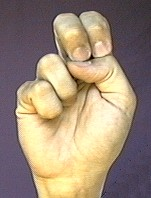
\includegraphics[scale=0.5]{images/e2.jpg}

There is even a version of ``E'' that uses only ``one'' finger (the index finger perched on top of the thumb).
This version often shows up after the letter ``L.''
None of these variations changes the symbol used to write the ``E'', just like you still spell ``input'' even if a particular speaker says something more like ``i{\footnotesize nm}put.''
The particular ``E'' used is not a separate letter, it's just a part of that signer's accent!

Note:
Sometimes you'll see people do an ``e'' with an opening between the fingertips and the thumb.
I sometimes call that a ``screaming E'' or a ``Hearing person's E.''
(Some people call it a ``bear claw E.'')
However it is fairly common in the Deaf Community and even used by quite a few Deaf people.
I recommend that ASL teachers stay flexible --- just like Spanish teachers have accepted several forms of the ``d'' sound.
I also recommend we not consider it ``wrong'' but simply another version of ``E'' that shows up from time to time depending on the person's particular accent. 

\subsubsection{F:}

B511x515S1ce20489x485 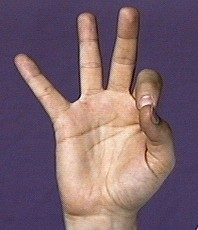
\includegraphics[scale=0.5]{images/f.jpg}

Tip:
Do ``not'' get hung up on debating if the tip of the finger is on top of the thumb or the pad of the index finger is on top of the thumb.
The exact form of an ``F'' varies a bit depending on surrounding letters.
However --- some people care ``a lot.''
If you have the unfortunate experience of being taught by such a person just smile and do it their way.

\subsubsection{G:}

B515x508S1f000486x493 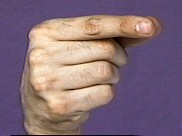
\includegraphics[scale=0.5]{images/g1.jpg} 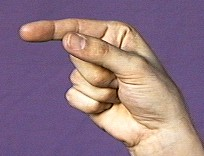
\includegraphics[scale=0.5]{images/g2.jpg}

You'll also see a ``G'' done with the thumb jutting up.
That is just another variation.

\subsubsection{H:}

B515x508S11502485x493 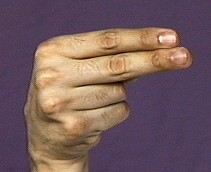
\includegraphics[scale=0.5]{images/h1.jpg} 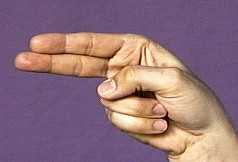
\includegraphics[scale=0.5]{images/h2.jpg} 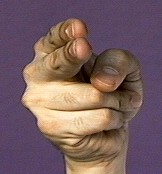
\includegraphics[scale=0.5]{images/h3.jpg}

You'll also see an ``H'' done with the thumb jutting up.
That is just another variation.
\subsubsection{I:}
\subsubsection{J:}

\subsubsection{K:}
\subsubsection{L:}
\subsubsection{M:}
\subsubsection{N:}
\subsubsection{O:}
\subsubsection{P:}
\subsubsection{Q:}
\subsubsection{R:}
\subsubsection{S:}
\subsubsection{I:}
\subsubsection{T:}
\subsubsection{U:}
\subsubsection{V:}
\subsubsection{W:}
\subsubsection{X:}
\subsubsection{Y:}
\subsubsection{Z:}
\begin{tabular}{p{1cm}p{14cm}}
\bul I know and can read the common handshapes used in ASL.\\

\bul I am able to read, write, and fingerspell my name in ASL.\\
\bul I am able to read, write, and count to five in ASL.\\
\bul I am able to briefly describe the history of ASL.\\
\bul I am able to briefly describe the history of SignWriting.\\
\bul I am able to briefly state the gist of Deaf Culture.\\
\bul I have a \emph{basic} idea of the meaning of the difference between ASL and Signed English.\\
\bul I have a \emph{basic} idea of the meaning of Pidgin (concat signing).\\
\bul I know which direction to read and write SignWriting.\\
\bul I am able to explain how the glyphs of SignWriting are organized.\\
B511x510S19220490x491 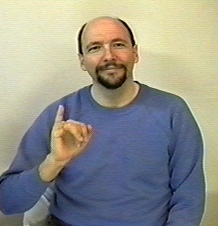
\includegraphics[scale=0.5]{images/i.jpg} 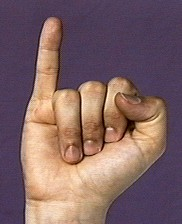
\includegraphics[scale=0.5]{images/i1.jpg}
\bul I have a \emph{basic} idea of how dictionary order works.\\
\bul I know how SignWriting works with left handed signing.\\
\bul I am able to read, recognize, and sign the vocabulary for this lesson.\\
\bul I am able to read, recognize, and sign the practice sentences for this lesson.\\
\bul I am able to read the practice story for this lesson.\\
\bul I have done a practice quiz.\\
\bul I have checked with my instructor regarding how and where to take any graded quizzez.\\
\end{tabular}
\begin{center}\textbf{\Huge This is where we are!}\end{center}\end{document}
<hr color="#800080">
<b>J</b>:<br>
<img border="0" src="../signjpegs/j/j1.jpg" width="214" height="230">
<img border="0" src="../signjpegs/j/j2.jpg" width="214" height="230">
<br>
&nbsp;
<img border="0" src="../signjpegs/j/j3.jpg" width="214" height="230">
<img border="0" src="../signjpegs/j/j4.jpg" width="214" height="230">
<br>
&nbsp;
<img border="0" src="../signjpegs/j/j5.jpg" width="214" height="230">
<img border="0" src="../signjpegs/j/j6.jpg" width="214" height="230">
<br>
&nbsp;
<img border="0" src="../signjpegs/j/j7.jpg" width="214" height="230">
<img border="0" src="../signjpegs/j/j8.jpg" width="214" height="230">
<br>
&nbsp;
<img border="0" src="../signjpegs/j/j9.jpg" width="214" height="230">
<img border="0" src="../signjpegs/j/j10.jpg" width="214" height="230">
<br>
&nbsp;
<img border="0" src="../signjpegs/j/j11.jpg" width="214" height="230"><img border="0" src="../signjpegs/j/j12.jpg" width="214" height="230">
<hr color="#800080">
<b>K</b>: <br>
<img border="0" src="../signjpegs/k/k.jpg" width="192" height="236"><img border="0" src="../signjpegs/k/k1.jpg" width="191" height="234"><br>
<img border="0" src="../signjpegs/k/k2.jpg" width="168" height="238">
<hr color="#800080">
<b>L</b>:<br>
<img border="0" src="../signjpegs/l/l.jpg" width="225" height="233">
<hr color="#800080">
<b>M</b>:&nbsp; Three fingers draped over the thumb.<br>
<img border="0" src="../signjpegs/m/m1.jpg" width="159" height="164"><br>
			<br>
In books you often see the fingers draped way over the thumb, like this:<br>
<img border="0" src="../signjpegs/m/m2.jpg" width="161" height="158"><br>
			<br>
			<font face="Arial">You'll see it both ways, but think about which 
			version would naturally become more popular over
the years due to ease of use..&nbsp; It takes extra time to drape the fingers
further over the thumb.&nbsp; So you can see why the &quot;loose method&quot; is
more popular amongst everyday users of ASL.</font><p><font face="Arial">When 
			most skilled signers fingerspell letters like
  &quot;M, N, &amp; T,&quot; they don't bend or wrap the fingers as tightly as the &quot;ABC&quot; alphabet charts tend to
  depict. The same for not bending the thumb over the palm in the letter &quot;B.&quot;&nbsp; Tightly wrapping the fingers over and/or around each other takes too much time. An artist has a
  long time to draw
  pretty handshapes.&nbsp; The artist can paint them carefully and in perfect form for the 
  sign language dictionary pages. A Deaf
  person whips out a several letters per second because he is trying to get his message
  across rather than impress somebody with how pretty his handshapes are.</font></p>
<hr color="#800080">
<b>N</b>:&nbsp; Version 1:<br>
<img border="0" src="../signjpegs/n/n1.jpg" width="154" height="197"><br>
<br>
Version 2:<br>
<img border="0" src="../signjpegs/n/n2.jpg" width="161" height="184">
<hr color="#800080">
<b>O</b>:<br>
&nbsp;<img border="0" src="../signjpegs/o/o.jpg" width="218" height="226"><img border="0" src="../signjpegs/o/o1.jpg" width="159" height="178"><br>
<img border="0" src="../signjpegs/o/o2.jpg" width="143" height="187"><img border="0" src="../signjpegs/o/o3.jpg" width="168" height="198"><hr color="#800080">
<b>P</b>:<br>
<img border="0" src="../signjpegs/p/p1.jpg" width="225" height="193"><img border="0" src="../signjpegs/p/p2.jpg" width="272" height="182"><br>
In some parts of the country you will see a &quot;p&quot; done like this:<br>
<img border="0" src="../signjpegs/p/p3.jpg" width="235" height="171">
<hr color="#800080">
<b>Q</b>:<br>
<img border="0" src="../signjpegs/q/q1.jpg" width="154" height="157"><img border="0" src="../signjpegs/q/q2.jpg" width="242" height="206">
<hr color="#800080">
<b>R</b>:<br>
<img border="0" src="../signjpegs/r/r.jpg" width="134" height="210">
<hr color="#800080">
<b>S</b>:<br>
<img border="0" src="../signjpegs/s/s.jpg" width="137" height="149">
<hr color="#800080">
<b>T</b>:<br>
<img border="0" src="../signjpegs/t/t.jpg" width="146" height="165">
<hr color="#800080">
<b>U</b>:<br>
<img border="0" src="../signjpegs/u/u.jpg" width="143" height="226">
<hr color="#800080">
<b>V</b>:<br>
<img border="0" src="../signjpegs/v/v.jpg" width="153" height="217"><br>
&nbsp;<hr color="#800080">
<b>W</b>:<br>
<img border="0" src="../signjpegs/w/w.jpg" width="173" height="224">
<hr color="#800080">
<b>X</b>:<br>
<img border="0" src="../signjpegs/x/x1.jpg" width="148" height="188"><img border="0" src="../signjpegs/x/x2.jpg" width="160" height="177">
<hr color="#800080">
<b>Y</b>:<br>
<img border="0" src="../signjpegs/y/y.jpg" width="245" height="191">
<hr color="#800080">
<b>Z</b>:<br>
&nbsp;<img border="0" src="../images-signs/z.gif" width="140" height="219"><br>
&nbsp;<hr>
<p>
<b>
Bent V handshape</b>:&nbsp;&nbsp;<br>
Uses: Things with legs, people and animals that are crouching, small animals<br>
Examples:&nbsp;<br>
- a small animal such as a squirrel <br>
- a person sitting in a certain location (when done palm facing downward)<br>
<br>
<img border="0" src="../signjpegs/v/v-bent.jpg" width="152" height="220">
<br>
A &quot;Bent V&quot; is also good for doing a &quot;double z.&quot;&nbsp; </p>
<hr color="#800080">
<b>
Bent hand</b>:<br>
<img border="0" src="../signjpegs/b/benthandshape.jpg" width="187" height="198"><img border="0" src="../signjpegs/b/benthandshape2.jpg" width="175" height="155">
<hr color="#800080">
<b>
Claw hand</b>:<br>
<img border="0" src="../signjpegs/c/claw.jpg" width="214" height="216">
<hr color="#800080">
<b>
Closed hand</b>:
<p>Fist or &quot;S hand&quot; or &quot;closed hand&quot;</p>
<p>
<img border="0" src="../signjpegs/s/s.jpg" width="137" height="149"></p>
<hr color="#800080">
<b>Curved hand</b>:<br>
<img border="0" src="../signjpegs/c/curvedhandshape.jpg" width="146" height="192"><img border="0" src="../signjpegs/c/curvedhandshape2.jpg" width="148" height="217">
<hr color="#800080">
<br><b>Horns</b>: <br>
  <img border="0" src="../signjpegs/h/horns1.jpg" width="160" height="235"><img border="0" src="../signjpegs/h/horns2.jpg" width="240" height="195"><hr color="#800080">
<b>Index</b>:<br>
			<img border="0" src="../signjpegs/i/indexfingerb.jpg" width="170" height="227"><br>
Cocked Index:<br>
<img border="0" src="../signjpegs/c/cockedindexfinger.jpg" width="147" height="211">
<hr color="#800080">
<b>
&quot;Open hand&quot; or &quot;5 hand&quot;<br>
&nbsp;<img border="0" src="../signjpegs/numbers/5.jpg" width="258" height="232"></b>

		</blockquote>
		<!--webbot bot="Include" U-Include="adsense1.htm" TAG="BODY" startspan -->
<blockquote>
<hr>
<p style="margin-top: 0; margin-bottom: 0">
<font size="2"><br>
NEW!&nbsp; Online &quot;<b>ASL Training Center!</b>&quot;&nbsp; (Premium Subscription Version of ASLU)&nbsp; **
	<a rel="nofollow" target="_blank" href="http://www.asl.tc/landing/index.html">CHECK IT OUT</a> **</font></p>
<p style="margin-top: 0; margin-bottom: 0">
<br>
<font size="2">Also available: &quot;ASLUniversity.com&quot; (a <i>mirror</i> of Lifeprint.com 
less traffic, fast access)&nbsp; **
<a rel="nofollow" target="_blank" href="http://asluniversity.com">VISIT NOW</a> **</font></p>
<form action="https://www.paypal.com/cgi-bin/webscr" method="post">
<font face="Arial">
<input type="hidden" name="cmd" value="_s-xclick">
<input type="hidden" name="hosted_button_id" value="AVN6HZ7MF9WVS">
</font>
<p align="left"><font size="2" face="Arial">Want to help support Lifeprint / ASLU?&nbsp; 
It's <i>easy! </i> </font><font face="Arial"><font size="2">&nbsp;&nbsp; </font>
<input type="image" src="https://www.paypalobjects.com/en_US/i/btn/btn_donate_LG.gif" border="0" name="submit" alt="PayPal - The safer, easier way to pay online!" align="texttop">
<font size="2">&nbsp;</font></font></p>
</form>

<p align="left" style="margin-top: 0; margin-bottom: 0">
<font face="Arial">
	<script type="text/javascript"><!--
google_ad_client = "ca-pub-2513564923850231";
/* topics-adsense1-bottom */
google_ad_slot = "8799753422";
google_ad_width = 728;
google_ad_height = 90;
//-->
</script>
<script type="text/javascript"
src="//pagead2.googlesyndication.com/pagead/show_ads.js">
</script>

<p align="center"></p>

	<script type="text/javascript"><!--
google_ad_client = "ca-pub-2513564923850231";
/* topics-adsense1-bottom */
google_ad_slot = "8799753422";
google_ad_width = 728;
google_ad_height = 90;
//-->
</script>
<script type="text/javascript"
src="//pagead2.googlesyndication.com/pagead/show_ads.js">
</script>

<p align="center"></p>

	<script type="text/javascript"><!--
google_ad_client = "ca-pub-2513564923850231";
/* topics-adsense1-bottom */
google_ad_slot = "8799753422";
google_ad_width = 728;
google_ad_height = 90;
//-->
</script>
<script type="text/javascript"
src="//pagead2.googlesyndication.com/pagead/show_ads.js">
</script>

<p align="center"></p>

<p style="margin-top: 0; margin-bottom: 0">
	<script type="text/javascript"><!--
google_ad_client = "ca-pub-2513564923850231";
/* 728x15_link_ads_adsense1_bottom */
google_ad_slot = "2289748297";
google_ad_width = 728;
google_ad_height = 15;
//-->
</script>
<script type="text/javascript"
src="//pagead2.googlesyndication.com/pagead/show_ads.js">
</script>
<p align="center" style="margin-top: 0; margin-bottom: 0"></p>

<script type="text/javascript"><!--
google_ad_client = "ca-pub-2513564923850231";
/* 728x15_link_ads_adsense1_bottom */
google_ad_slot = "2289748297";
google_ad_width = 728;
google_ad_height = 15;
//-->
</script>
<script type="text/javascript"
src="//pagead2.googlesyndication.com/pagead/show_ads.js">
</script>
<p align="center" style="margin-top: 0; margin-bottom: 0"></p>


<script type="text/javascript"><!--
google_ad_client = "ca-pub-2513564923850231";
/* 728x15_link_ads_adsense1_bottom */
google_ad_slot = "2289748297";
google_ad_width = 728;
google_ad_height = 15;
//-->
</script>
<script type="text/javascript"
src="//pagead2.googlesyndication.com/pagead/show_ads.js">
</script>

</p></font>
</blockquote><!--webbot bot="Include" i-checksum="23068" endspan --></td>
		<td align="right" width="160" valign="top">
		<!--webbot bot="Include" U-Include="adsense2.htm" TAG="BODY" startspan -->
<!--webbot bot="Include" i-checksum="32" endspan --></td>
	</tr>
	</table>
<p align="left" style="margin-top: 0; margin-bottom: 0"></p>
	
</body>

</html>
\subsection{The Common Handshapes of ASL}

\begin{center}
\large
\begin{tabular}{*{3}{c}}
\textbf{Bent V}&\textbf{Bent Hand}&\textbf{Claw Hand}\\
B508x514S11000493x487&B512x508S14b00489x493&B513x516S15000488x485\\
\textbf{Closed Hand}&\textbf{Curved Hand}&\textbf{Horns}\\
B508x508S20300493x493&B512x510S16e00489x490&B510x515S1a000490x486\\
\textbf{Index}&\textbf{Cocked Index}&\textbf{Open Hand}\\
B508x515S10000493x485&B508x510S10900493x490&B512x516S14c00489x485\\
\end{tabular}
\end{center}

\subsection{Writing Your Name In SignWriting}

Take a small peek into supplement 2 for a list of symbols for fingerspelling.
With how visual SignWriting is, you can start by just ``drawing'' them while remembering:

\begin{tabular}{p{1cm}p{14cm}}
\bul keep the letters centered in a column;\\
\bul for each hand, draw the palm with it's fill;\\
\bul then decorate each palm with fingers.\\
\end{tabular}

\subsection{The Numbers One Through Five}

\begin{center}
\large
\begin{tabular}{*{5}{c}}
\textbf{One}&\textbf{Two}&\textbf{Three}&\textbf{Four}&\textbf{Five}\\
B508x515S10000493x485&B508x515S10e00493x485&B512x515S11e00489x485&B511x516S14400489x485&B512x516S14c00489x485\\
\end{tabular}
\end{center}

\subsection{A Very Brief History of SignWriting}

\begin{quote}
\begin{center}
\emph{This is almost an extract from \emph{www.signwriting.org/library/history}.}

\emph{Please feel free to do some additional reading.}
\end{center}
\end{quote}

Valerie Sutton invented a notation to record the movements of ballet as part of her dance studies.
She then movend to Copenhagen to train in the Danish Royal Ballet and began to record their movements to prevent the loss of ballet through time.
Some people researching Danish Sign Language read a newspaper article about it and contacted her to record the movements of signing---this became the earliest form of SignWriting.

When Valerie Sutton returned home her research turned to recording ASL.
Soon books, articles, pamphlets, and even a newsletter began to be written in ASL using SignWriting.
Then SignWriting began to be put into a computer, and with that SignWriting became simplified, abstract, and regular.

It was during this time that Deaf users of SignWriting demanded that SignWriting switch from recording what a researcher sees (receptive) to what a signer does (expressive).
Then the direction changed from horizontal to vertical.

Today it is used for close to sixty sign languages, with more than a dozen langugae codes, and is the official writing system for Brazilian Sign Language.

\subsection{Direction of Reading and Writing}

A full word in ASL can consist of a face along with movement and handshapes that change over the course of movement.
If SignWriting is written horizontally, as it was initially, then you are left with a word which is half iconic with individual parts of the word being iconic but thos parts being horizontally separated from eachother.
So, of course, inidivdual words have long been written vertically even if the words were strung along horizontally.

Along with writing ASL came a better understanding of the grammar of ASL and a way to write role shifting was required.
The simplest way to accomplish this?
Write the words vertically and place them in the correct column corresponding to the role.

Today all SignWriting is written vertically, from the top of the page to the bottom of the page, with columns of text moving from the left of the page to the top ef the page.

\subsection{How Do I Remember Over 10,000 Letters?}

Yes, that is correct.
SignWriting has about ten thousand ``letters'', though there are a couple things that make this less daunting.

The first thing to remember is that ASL doesn't use every letter, just like even if English was written in the International Phonetic Alphabet it would not require all hundred or so letters.
SignWriting is usable for all sign languages, and even though we will be learning \emph{about} the whole system we will focus on the \emph{part} that ASL uses.

The second thing to know is that SignWriting isn't just a list of ten thousand letters, but organized into related groups.
So when you see B516x515S14521484x485, its not just \emph{symbol 7,520.}
It's \emph{Category One, Symbol Group Four Fingers, Second Symbol, Fill Three, Rotation One}.

The levels of organization for SignWriting are:

\begin{tabular}{p{1cm}p{14cm}}
\hfil 1.&\textbf{Category.}
Every symbol in SignWriting fits into one of these seven categories.\\
\hfil 2.&\textbf{Symbol group.}
Each category has between one and ten symbol groups for a total of thirty symbol groups which you will eventually know as well as you know your own alphabet.\\
\hfil 3.&\textbf{Base symbol.}
Each symbol group has a number of base symbols, the closest thing corresponding to a letter.\\
\hfil 4.&\textbf{Fill}.
Each base symbol has between one and six fills.\\
\hfil 5.&\textbf{Rotation}.
Each fill has between one and sixteen different rotations, though it tends to be regular enough that it can be ignored when identifying a symbol.\\
\end{tabular}

\subsection{The Basics of Dictionary Order}

Let's start by comparing the order of our glossary with the order of a typical English dictionary.

\begin{tabular}{p{1mm}*{2}{p{7cm}}}
1.&
Even if you don't know whether \# comes before \emph{apple} or after \emph{zebra} you know that punctuation marks will be grouped together.&
SignWriting symbols are grouped by their functional categories.\\
2.&
Alphabetic order is arbitrary. The letter \emph{A} comes before \emph{B} simply because of where the Romans borrowed them from.&
The order is arbitrary, someone picked it.\\
3.&
The exact rules being followed vary slightly on purpose. For instance, author lists will treat \emph{Mac} and \emph{Mc} as a separate letter between \emph{M} and \emph{N}.&
This sorting follows the international standard but you may find different ways to sort in other places.\\
4.&
We sort word by word so \emph{I Read} comes before \emph{In May}.&
These rules are for sorting words.\\
5.&
Shorter words come before longer words so \emph{pen} comes before \emph{penmanship}.&
% I can't seem to use \f@size in a raisbox!
Words like \raisebox{-4mm}{{\setmainfont{SuttonSignWritingLine.ttf}\fontsize{10pt}{10pt}\selectfont\begin{tikzpicture}\draw(10/30*0 pt,10/30*1 pt) node [anchor=north west] {\char983049};\draw(10/30*6 pt,10/30*-6 pt) node [anchor=north west] {\char983073};\draw(10/30*5 pt,10/30*-41 pt) node [anchor=north west] {\char1017409};\end{tikzpicture}}} come before words like \raisebox{-5mm}{{\setmainfont{SuttonSignWritingLine.ttf}\fontsize{10pt}{10pt}\selectfont\begin{tikzpicture}\draw(10/30*0 pt,10/30*-31 pt) node [anchor=north west] {\char983049};\draw(10/30*6 pt,10/30*-38 pt) node [anchor=north west] {\char983073};\draw(10/30*5 pt,10/30*-73 pt) node [anchor=north west] {\char1017409};\draw(10/30*1 pt,10/30*0 pt) node [anchor=north west] {\char1017429};\end{tikzpicture}}}.\\
\end{tabular}

For English, that's the end of the story because one sound comes at a time; but in ASL more than one thing can be happening at the same time so we have to decide how to handle both simultaneous and sequential activity.
A full sign is first broken into syllables based generally on sequential ordering.

B566x629S30a00482x483S11817490x522S15a06487x555S2970b515x543S15a36533x617S20b00553x599S10e30530x593 \raisebox{9mm}{becomes}
\begin{tabular}{p{1cm}p{11cm}}
\hfil 1.&\textbf{Syllable 1.}
Hands beginning position --- B514x523S11817489x478S15a06486x511\\
\hfil 2.&\textbf{Syllable 2.}
Movement between hand positions --- {B526x535S2970b475x466S20b00513x522}\\
\hfil 3.&\textbf{Syllable 3.}
Hands ending position --- {B515x518S15a36488x506S10e30485x482}\\
\hfil 4.&\textbf{Syllable 4.}
Everything else --- {B518x518S30a00482x483}\\
\end{tabular}

For longer or compound words we extend this pattern---hand shapes, movement, handshapes, movement, $\ldots$, handshapes, everything else.
Then within each of these syllables we consider all the simultaneous things that can occur in a certain order.

For odd syllables we sort the right hand (\raisebox{3mm}{\setmainfont{SuttonSignWritingLine.ttf}\char985368}, \raisebox{3mm}{\setmainfont{SuttonSignWritingLine.ttf}\char984433}), then the left (\raisebox{2mm}{\setmainfont{SuttonSignWritingLine.ttf}\char991687}, \raisebox{2mm}{\setmainfont{SuttonSignWritingLine.ttf}\char991735}).

For even syllables, except the last, we sort right hand movement (\raisebox{3mm}{\setmainfont{SuttonSignWritingLine.ttf}\char1022124}), simultaneous movement (\raisebox{2mm}{\setmainfont{SuttonSignWritingLine.ttf}\char1008673}), and finally left hand movement.

For the last syllable we just follow the arbitrary order we will be learning over the next several supplements.

\subsection{SignWriting and Left Handed Signing}

Throughout these lessons I refer to right and left hands.
It would be most accurate to call them dominant and non-dominant hands.
When using SignWriting to read ASL the dominant hand visually appears as if it is the right hand and is placed on the right side.

Of course, for your own writing you are free to draw the sign anyway you would prefer, but for purposes of these supplements we assume right-handed signers.

\subsection{Vocabulary for Lesson 1}

\begin{glossary}
\textbf{1}\\
AS10000M508x515S10000493x485

\textbf{2}\\
AS10e00M508x515S10e00493x485

\textbf{3}\\
AS11e00M512x515S11e00489x485

\textbf{4}\\
AS14400M511x516S14400489x485

\textbf{5}\\
AS14c00M512x516S14c00489x485

\textbf{again}\\
AS18250S15a39S28801S20500M530x516S15a39471x488S20500499x484S18250480x501S28801510x493

\textbf{clean}\\
AS15a51S15a37S26507S21100M528x522S15a37473x486S15a51482x499S26507515x479S21100500x492

\textbf{deaf}\\
AS10011S20500S20500S2ff00M544x531S20500509x515S10011523x501S20500520x488S2ff00482x483

\textbf{don't understand}\\
AS10000S21c00S30122M537x524S30122482x476S10000520x476S21c00531x465

\textbf{hearing}\\
AS10012S2ea08S2ff00M533x549S2ff00482x483S2ea08491x524S10012503x508

\textbf{learn}\\
AS14c51S15a37S20500S22c00S18510S20500S2ff00M543x567S15a37482x526S14c51500x541S22c00520x503S20500512x467S18510518x482S2ff00482x483S20500488x533

\textbf{like (emotion)}\\
AS14c02S20e00S26500S1bb02M516x540S1bb02488x461S14c02484x517S20e00499x502S26500499x483

\textbf{meaning}\\
AS10e22S15a18S20500S10e02S15a18S20500M522x542S15a18478x464S10e22492x471S15a18478x506S10e02492x514S20500492x459S20500492x531

\textbf{meet}\\
AS10020S10008S26600S26614S20500M514x552S10008486x480S10020492x487S20500504x485S26614487x449S26600491x522

\textbf{name}\\
AS11541S11549S20600M522x525S11541498x491S11549479x498S20600489x476

\textbf{nice}\\
AS15a51S15a37S26507S21100M528x522S15a37473x486S15a51482x499S26507515x479S21100500x492

\textbf{no}\\
AS13f10S22114M516x513S13f10487x498S22114484x487

\textbf{over}\\%again
AS18250S15a39S28801S20500M530x516S15a39471x488S20500499x484S18250480x501S28801510x493

\textbf{public}\\%hearing
AS10012S2ea08S2ff00M533x549S2ff00482x483S2ea08491x524S10012503x508

\textbf{repeat}\\%again
AS18250S15a39S28801S20500M530x516S15a39471x488S20500499x484S18250480x501S28801510x493

\textbf{re-}\\%again
AS18250S15a39S28801S20500M530x516S15a39471x488S20500499x484S18250480x501S28801510x493

\textbf{say}\\%hearing
AS10012S2ea08S2ff00M533x549S2ff00482x483S2ea08491x524S10012503x508

\textbf{sign (as in ``signing'')}\\
AS10011S10019S2ea04S2ea48M523x535S2ea48483x510S10011502x466S2ea04508x500S10019477x475

\textbf{slow}\\
AS15a51S15a50S21100S26504M523x524S26503497x511S21100490x497S15a57477x476S15a51500x481

\textbf{speak}\\%hearing
AS10012S2ea08S2ff00M533x549S2ff00482x483S2ea08491x524S10012503x508

\textbf{student}\\
AS14c51S15a37S20500S22c00S18510S20500S15a40S15a48S22a24S2ff00M543x638S15a37480x556S14c51501x539S22c00520x503S20500512x467S18510518x482S2ff00482x483S20500487x562S15a40509x591S15a48482x590S22a24494x623

\textbf{teacher}\\
AS18510S18518S26500S26510S15a40S15a48S22a24S2ff00M546x575S2ff00482x483S18510521x490S18518452x493S26500525x468S26510458x469S15a40507x524S15a48481x525S22a24493x560

\textbf{thank you}\\
AS15a00S26500S2ff00M535x536S26500521x498S2ff00482x483S15a00495x509

\textbf{understand}\\
AS10000S21b00S2ff00M536x518S2ff00482x483S10000520x471S21c00530x461

\textbf{what}\\
AS14c31S14c39S26c0aS26c12S2fb04M553x518S2fb04492x512S26c0a538x483S26c12448x488S14c39468x483S14c31506x483

\textbf{where}\%\
AS10020S27106M518x525S10020482x476S27106503x485

\textbf{who}\\
AS1e111S21800S34600M518x540S34600482x483S1e111473x512S21800463x502

\textbf{why}\\
AS15d11S22a05S19a37S2ff00M574x535S22a05540x506S15d11520x488S19a37551x508S2ff00482x483

\textbf{yes}\\
AS20320S23004M513x519S20320493x482S23004488x501

\textbf{\emph{Indexing}}

\textbf{he}\\
AS10047S26507M515x519S10047485x498S26507501x481

\textbf{her}\\
AS10047S26507M515x519S10047485x498S26507501x481

\textbf{him}\\
AS10047S26507M515x519S10047485x498S26507501x481

\textbf{I}\\
AS10043S20500M518x518S10043488x483S20500482x507

\textbf{it}\\
AS10047S26507M515x519S10047485x498S26507501x481

\textbf{me}\\
AS10043S20500M518x518S10043488x483S20500482x507

\textbf{she}\\
AS10047S26507M515x519S10047485x498S26507501x481

\textbf{you}\\
AS10040S26500M510x523S10040495x493S26500491x478

\textbf{\emph{Plural Indexing}}

\textbf{them}\\
AS10047S2d608M529x519S10047471x498S2d608500x482

\textbf{they}\\
AS10047S2d608M529x519S10047471x498S2d608500x482

\textbf{us}\\
AS10043S2d600M531x511S10043501x489S2d600469x499

\textbf{we}\\
AS10043S2d600M531x511S10043501x489S2d600469x499

\textbf{you}\\
AS10040S2d608M520x524S10040481x494S2d608491x477

\textbf{\emph{Possesive Indexing}}

\textbf{hers}\\
AS15a20S26507M513x520S15a20487x493S26507500x481

\textbf{his}\\
AS15a20S26507M513x520S15a20487x493S26507500x481

\textbf{its}\\
AS15a20S26507M513x520S15a20487x493S26507500x481

\textbf{mine}\\
AS15a01S20500M513x514S15a01490x486S20500487x503

\textbf{my}\\
AS15a01S20500M513x514S15a01490x486S20500487x503

\textbf{your}\\
AS15a20S26500M507x523S15a28494x496S26500493x477

\textbf{yours}\\
AS15a20S26500M507x523S15a28494x496S26500493x477

\end{glossary}

\subsection{Practice Sheet 1.A}

\begin{multicols}{5}
\begin{center}
M508x515S10000493x485 % 1
M536x504S38800464x496 % .
M510x523S10040495x493S26500491x478 % you
M518x518S30c00482x483 % \?
M522x525S11541498x491S11549479x498S20600489x476 % name
M536x507S38900464x493 % ?
\vfil
\columnbreak

M508x515S10e00493x485 % 2
M536x504S38800464x496 % .
M544x531S20500509x515S10011523x501S20500520x488S2ff00482x483 % deaf
M518x518S30a00482x483 % y/n
M510x523S10040495x493S26500491x478 % you
M536x507S38900464x493 % ?
\vfil
\columnbreak

M512x515S11e00489x485 % 3
M536x504S38800464x496 % .
M543x638S15a37480x556S14c51501x539S22c00520x503S20500512x467S18510518x482S2ff00482x483S20500487x562S15a40509x591S15a48482x590S22a24494x623 % student
M518x518S30a00482x483 % y/n
M510x523S10040495x493S26500491x478 % you
M536x507S38900464x493 % ?
\vfil
\columnbreak

M511x516S14400489x485 % 4
M536x504S38800464x496 % .
M511x516S14400489x485 % your
M546x575S2ff00482x483S18510521x490S18518452x493S26500525x468S26510458x469S15a40507x524S15a48481x525S22a24493x560 % teacher
M518x518S30c00482x483 % \?
M522x525S11541498x491S11549479x498S20600489x476 % name
M536x507S38900464x493 % ?
\vfil
\columnbreak

M512x516S14c00489x485 % 5
M536x504S38800464x496 % .
M510x523S10040495x493S26500491x478 % you
M536x518S2ff00482x483S10000520x471S21c00530x461 % understand
M518x518S30a00482x483 % y/n
M515x519S10047485x498S26507501x481 % 3rd person
M536x507S38900464x493 % ?
\vfil

\end{center}
\end{multicols}

\subsection{Practice Sheet 1.B}

\begin{multicols}{5}
\begin{center}

M509x515S18720491x486 % 6
M536x504S38800464x496 % .
M515x519S10047485x498S26507501x481 % 3rd person
M518x540S34600482x483S1e111473x512S21800463x502S30c00482x483 % who?
M536x507S38900464x493 % ?
\vfil
\columnbreak

M511x514S1a520490x486 % 7
M536x504S38800464x496 % .
M530x516S15a39471x488S20500499x484S18250480x501S28801510x493 % again
M537x504S38700463x496 % ,
M510x523S10040495x493S26500491x478 % you
M518x518S30c00482x483 % \?
M522x525S11541498x491S11549479x498S20600489x476 % name
M536x507S38900464x493 % ?
\vfil
\columnbreak

M511x514S1bb20490x486 % 8
M536x504S38800464x496 % .
M515x519S10047485x498S26507501x481 % 3rd person
M543x638S15a37480x556S14c51501x539S22c00520x503S20500512x467S18510518x482S2ff00482x483S20500487x562S15a40509x591S15a48482x590S22a24494x623 % student
M518x518S30a00482x483 % y/n
M515x519S10047485x498S26507501x481 % 3rd person
M536x507S38900464x493 % ?
\vfil
\columnbreak

M511x515S1ce20489x485 % 9
M536x504S38800464x496 % .
M515x519S10047485x498S26507501x481 % 3rd person
M518x518S30a00482x483 % y/n
M511x516S14400489x485 % your
M536x507S38900464x493 % ?
\vfil
\columnbreak

M513x528S2a538494x472S1f540488x504 % 10
M536x504S38800464x496 % .
M536x511S38a00464x490 % :
M536x511S38a00464x490 % :
M518x518S30c00482x483 % \?
M518x525S10020482x476S27106503x485 % where
M536x507S38900464x493 % ?
\vfil

\end{center}
\end{multicols}

\subsection{Practice Sheet 1.C}
\begin{multicols}{5}
\begin{center}


M512x520S10000489x490S21d00494x480 % 11
M536x504S38800464x496 % .
M528x522S15a37473x486S15a51482x499S26507515x479S21100500x492 % nice
M514x536S10008486x464S10020492x471S20500504x469S26600491x506 % meet you
M536x504S38800464x496 % .
\vfil
\columnbreak

M509x521S10e00491x491S21d00491x480 % twelve
M536x504S38800464x496 % .
M533x549S2ff00482x483S2ea08491x524S10012503x508 % hearing
M518x518S30a00482x483 % y/n
M510x523S10040495x493S26500491x478 % you
M536x507S38900464x493 % ?
\vfil
\columnbreak

M513x519S22114487x481S12d00489x489 % 13
M536x504S38800464x496 % .
M510x508S1f720490x493 % a (letter)
M508x508S20320493x493 % s
M512x515S1dc20488x485 % l
M546x575S2ff00482x483S18510521x490S18518452x493S26500525x468S26510458x469S15a40507x524S15a48481x525S22a24493x560 % teacher
M518x518S30a00482x483 % y/n
M510x523S10040495x493S26500491x478 % you
M536x507S38900464x493 % ?
\vfil
\columnbreak

M513x515S14700493x493S22114487x486 % 14
M536x504S38800464x496 % .
M510x523S10040495x493S26500491x478 % you
M543x567S15a37482x526S14c51500x541S22c00520x503S20500512x467S18510518x482S2ff00482x483S20500488x533 % learn
M523x535S2ea48483x510S10011502x466S2ea04508x500S10019477x475 % sign (as in ``signing'')
M537x504S38700463x496 % ,
M518x518S30c00482x483 % \?
M518x525S10020482x476S27106503x485 % where
M536x507S38900464x493 % ?
\vfil
\columnbreak

M513x518S22114487x483S15d00494x491 % 15
M536x504S38800464x496 % .
M510x523S10040495x493S26500491x478 % you
M543x567S15a37482x526S14c51500x541S22c00520x503S20500512x467S18510518x482S2ff00482x483S20500488x533 % learn
M523x535S2ea48483x510S10011502x466S2ea04508x500S10019477x475 % sign (as in ``signing'')
M537x504S38700463x496 % ,
M574x535S22a05540x506S15d11520x488S19a37551x508S30c00482x483 % why?
M536x507S38900464x493 % ?
\vfil

\end{center}
\end{multicols}

\subsection{Practice Sheet 1.D}
\begin{multicols}{5}
\begin{center}

M520x522S18700502x492S2e00e480x479 % 16
M536x504S38800464x496 % .
M508x510S1fb20493x491 % t
M515x508S11502485x493 % h
M510x508S1f720490x493 % a (letter)
M511x513S11920490x487 % n
M515x515S14020486x485 % k
M508x508S20320493x493 % s
M518x518S30c00482x483 % \?
M523x535S2ea48483x510S10011502x466S2ea04508x500S10019477x475 % sign (as in ``signing'')
M536x507S38900464x493 % ?
\vfil
\columnbreak

M522x522S1a500501x494S2e00e478x478 % 17
M536x504S38800464x496 % .
M543x638S15a37480x556S14c51501x539S22c00520x503S20500512x467S18510518x482S2ff00482x483S20500487x562S15a40509x591S15a48482x590S22a24494x623 % student
M537x504S38700463x496 % ,
M518x518S30a00482x483 % y/n
M515x519S10047485x498S26507501x481 % 3rd person
M536x507S38900464x493 % ?
\vfil
\columnbreak

M523x522S1bb00502x492S2e00e478x479 % 18
M536x504S38800464x496 % .
M518x518S30a00482x483 % y/n
M529x519S10047471x498S2d608500x482 % they
M543x567S15a37482x526S14c51500x541S22c00520x503S20500512x467S18510518x482S2ff00482x483S20500488x533 % learn
M523x535S2ea48483x510S10011502x466S2ea04508x500S10019477x475 % sign (as in ``signing'')
M536x507S38900464x493 % ?
\vfil
\columnbreak

M524x522S1ce00502x490S2e00e477x479 % 19
M536x504S38800464x496 % .
M511x516S14400489x485 % your
M546x575S2ff00482x483S18510521x490S18518452x493S26500525x468S26510458x469S15a40507x524S15a48481x525S22a24493x560 % teacher
M537x504S38700463x496 % ,
M518x540S34600482x483S1e111473x512S21800463x502S30c00482x483 % who?
M536x507S38900464x493 % ?
\vfil
\columnbreak

M517x513S22114484x488S1f420488x498 % 20
M536x504S38800464x496 % .
M510x523S10040495x493S26500491x478 % you
M518x518S30a00482x483 % y/n
M516x540S1bb02488x461S14c02484x517S20e00499x502S26500499x483 % like (emotion)
M543x567S15a37482x526S14c51500x541S22c00520x503S20500512x467S18510518x482S2ff00482x483S20500488x533 % learn
M523x535S2ea48483x510S10011502x466S2ea04508x500S10019477x475 % sign (as in ``signing'')
M536x507S38900464x493 % ?
\vfil

\end{center}
\end{multicols}

\subsection{Story 1}

\begin{multicols}{5}
\begin{center}
M547x518S2ff00482x483S22a07534x476S14711519x487 % hi
M518x518S10043488x483S20500482x507 % me
M536x511S38a00464x490 % :
M536x511S38a00464x490 % :
M536x504S38800464x496 % .

M528x522S15a37473x486S15a51482x499S26507515x479S21100500x492 % nice
M514x536S10008486x464S10020492x471S20500504x469S26600491x506 % meet you
M536x504S38800464x496 % .

M518x518S10043488x483S20500482x507 % me
M533x549S2ff00482x483S2ea08491x524S10012503x508 % hearing
M536x504S38800464x496 % .

M518x518S10043488x483S20500482x507 % me
M543x638S15a37480x556S14c51501x539S22c00520x503S20500512x467S18510518x482S2ff00482x483S20500487x562S15a40509x591S15a48482x590S22a24494x623 % student
M536x511S38a00464x490 % :
M536x511S38a00464x490 % :
M536x504S38800464x496 % .

M518x518S10043488x483S20500482x507 % me
M543x567S15a37482x526S14c51500x541S22c00520x503S20500512x467S18510518x482S2ff00482x483S20500488x533 % learn
M543x567S15a37482x526S14c51500x541S22c00520x503S20500512x467S18510518x482S2ff00482x483S20500488x533 % learn
M523x535S2ea48483x510S10011502x466S2ea04508x500S10019477x475 % sign (as in ``signing'')
M536x504S38800464x496 % .

M546x575S2ff00482x483S18510521x490S18518452x493S26500525x468S26510458x469S15a40507x524S15a48481x525S22a24493x560 % teacher
M522x525S11541498x491S11549479x498S20600489x476 % name
M536x511S38a00464x490 % :
M536x511S38a00464x490 % :
M536x504S38800464x496 % .

M515x519S10047485x498S26507501x481 % 3rd person
M544x531S20500509x515S10011523x501S20500520x488S2ff00482x483 % deaf
M525x525S38701475x475 % /
M526x520S11541474x481S2880a504x499S22a04492x505 % hard of hearing
M525x525S38701475x475 % /
M533x549S2ff00482x483S2ea08491x524S10012503x508 % hearing
M536x504S38800464x496 % .

M515x519S10047485x498S26507501x481 % 3rd person
M546x518S2ff00482x483S18510521x490S18518452x493S26500525x468S26510458x469 % teach
M518x604S15a31493x577S2ff00482x483S22b04492x538S15a37478x572S15a00495x507S20500490x593 % good
M536x504S38800464x496 % .

M518x518S10043488x483S20500482x507 % me
M536x518S2ff00482x483S10000520x471S21c00530x461 % understand
M515x519S10047485x498S26507501x481 % 3rd person
M536x504S38800464x496 % .

M518x518S10043488x483S20500482x507 % me
M516x540S1bb02488x461S14c02484x517S20e00499x502S26500499x483 % like (emotion)
M515x519S10047485x498S26507501x481 % 3rd person
\end{center}
\end{multicols}

\end{document}

